El primer nodo será el encargado principalmente de la actuación sobre distintos
elementos del sistema, a saber: el freno, las luces de cruce e indirectamente sobre
la alarma. Esto lo hará recogiendo datos de distintos sensores como son el velocímetro,
el sensor de distancia y el sensor de luminosidad para adecuar su comportamiento a las
circunstancias del entorno.

Este sistema contará con cuatro tareas en tiempo real y usará dos objetos protegidos:
el primero de ellos para conservar el valor de la velocidad actual; y el segundo para
guardar tanto el valor de la distancia con el vehículo precedente como la intensidad
del freno que se ha de aplicar en caso de peligro de colisión. Por su parte, las
tareas en cuestión son:

\begin{enumerate}
  \item \texttt{Cálculo velocidad} -- cada $\numprint[ms]{250}$, realizará una lectura
        del sensor en cuestión mediante el ADC y actualizará el valor del objeto 
        protegido \texttt{V\_actual}.
  \item \texttt{Cálculo distancia} -- cada $\numprint[ms]{300}$, el sistema obtendrá la
        distancia con el vehículo precedente usando el sensor de ultrasonidos y
        actualizará el valor del objeto protegido \texttt{D\_actual}. Además, leerá el
        valor de \texttt{V\_actual} y computará lo que sería la distancia de seguridad
        mínima que hay que respetar, descrita por la ecuación \ref{eq:min-dist}:

        \begin{equation}\label{eq:min-dist}
          d_{\min} = \left(\frac{V}{10}\right)^2,~\begin{cases}
            d_{\min} &: \text{distancia mínima que hay que mantener.} \\
            V &: \text{velocidad actual del vehículo.}
          \end{cases}
        \end{equation}

        En caso de que la distancia de seguridad no se cumpla (y según el valor relativo
        con que no se cumple), la tarea indicará en \texttt{Intens\_Frenada} con qué
        intensidad se ha de aplicar el freno para evitar una colisión. Finalmente,
        activará la tarea esporádica \texttt{Freno} para que realice su ejecución.
  \item \texttt{Freno} -- cada $\numprint[ms]{150}$ como mucho, realizará la activación
        progresiva del freno cada $\numprint[ms]{100}$ hasta alcanzar la intensidad
        apropiada. Al ser una tarea esporádica, depende directamente de la activación
        desde \texttt{Cálculo distancia}, lo cual añadirá un \textit{jitter} al tiempo
        de respuesta global de la tarea.
  \item \texttt{Luces de cruce} -- cada $\numprint[ms]{1000}$, el sistema realizará una
        valoración de la luminosidad del entorno y procederá a encender o apagar automáticamente
        las luces de cruce. Se establece que las luces se activarán si la intensidad lumínica
        está por debajo de $100$.
\end{enumerate}

Todo este sistema viene modelado por la figura \ref{fig:node1}:

\begin{figure}[H]
  \centering
  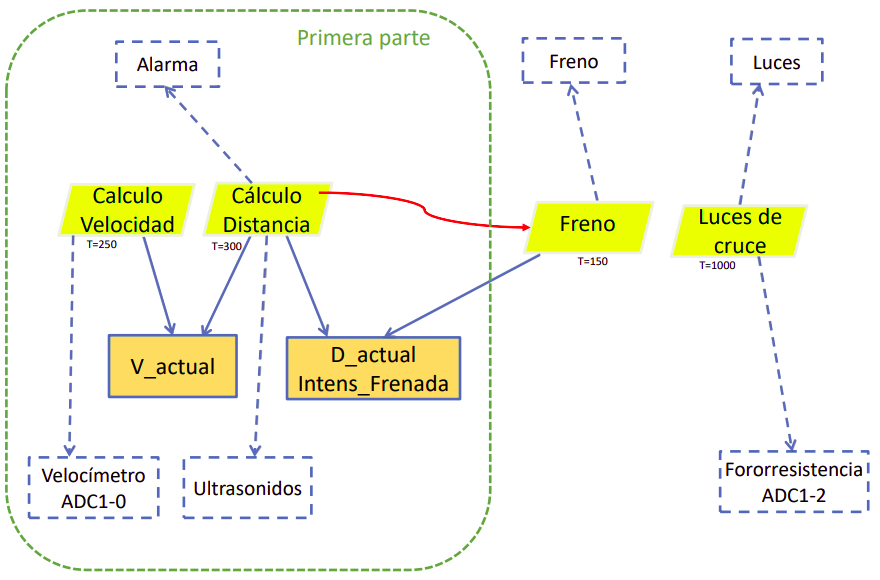
\includegraphics[width=.8\linewidth]{pictures/node1.png}
  \caption{Modelado del nodo 1 junto con sus tareas, objetos protegidos, sensores y actuadores.}
  \label{fig:node1}
\end{figure}